\documentclass[tikz,border=10pt]{standalone}
\usepackage{tikz}
\usepackage{amsmath,amssymb}
\usetikzlibrary{automata,backgrounds,shapes,arrows,positioning,calc,fit}
\usetikzlibrary{decorations,decorations.pathreplacing,decorations.pathmorphing,arrows.meta}

% Custom commands
\newcommand{\push}[1][]{\mathsf{push}_{#1}}
\newcommand{\pop}[1][]{\mathsf{pop}_{#1}}

\begin{document}
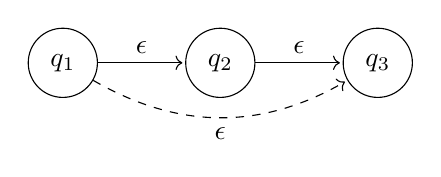
\begin{tikzpicture}[shorten >=1pt, node distance=2cm, on grid, auto]

  % States for the eps-eps diagram
  \node[state] (r1) at (0,0) {$q_1$};
  \node[state] (r2) [right=of r1] {$q_2$};
  \node[state] (r3) [right=of r2] {$q_3$};

  % Arrows for the eps-eps diagram
  \path[->]
    (r1) edge node {$\epsilon$} (r2)
    (r2) edge node {$\epsilon$} (r3)
    (r1) edge[bend right, dashed, swap] node {$\epsilon$} (r3);

\end{tikzpicture}
\end{document}